\documentclass{article}
\usepackage{hyperref}
\usepackage{graphicx} 

\title{Fuctional Secification\\Dynamic scheduling for scientific simulation}
\date{25.02.2015}
\author{Kai Bittner\\
		Ard Kastrati\\
		Fabio Broghammer\\
		Jan Ellmers\\
		David Krenz\\
		Benjamin-Philipp Roth}

\begin{document}
	\pagenumbering{gobble}	
	\maketitle
	\newpage
	\tableofcontents
	\newpage
	\pagenumbering{arabic}
	
	\section{Introduction}


%Die Anwendung wird in wissenschaftlichen Code eingebunden und verwaltet Ausführung einer gesamten Berechnung, die in einzelne tasks unterteilt ist. Tasks stellen hierbei einzelne Simulationsinstanzen mit spezifischen Parametern dar. Durch die Ausführung der tasks werden Metainformationen gespeichert, mit dem Ziel einen möglichst optimalen Programmfluss zu gewährleisten. Die gespeicherten Metainformationen werden von einem Datamining Modul ausgewertet. Daraus kann dynamisch zur Laufzeit der Berechnung die Laufzeit optimiert werden. Die aufgezeichneten Informationen können anschließend wahlweise grafisch ausgegeben werden.


%The application is meant to be linked into scientific code, functioning as runtime managing service for scientific simulations constisting of huge ammounts of tasks beeing single calculations unter specified changing parameters.
%Gathering meta informations about single calculation runs the schedular is able to use these to boost performance and throughtput of the whole scientific simulation. If chosen, the all data gathered can be plotted and put out graphically.


<<<<<<< HEAD
The application works as runtime administration service for scientific simulations. Linked into scientific code it manages huge computations consisting of large amounts of individual tasks. In this context tasks are specified as particular calculation runs with a given set of parameters. The scheduling module will load prestored data from the data base module and use it as initial information for scheduling. Gathering meta information about seperately performed calculations the schedular is able to dynamically adjust administration to increase performance of the whole computation. Obtained data can be plotted after the simulation is finished, if the user so chooses. In any case, it will be stored on a data base module to be used as initial information for scheduling calculation in future simulations.


The application to be developed works as runtime administration service for scientific simulations calculated on high performance comuters(HPCs) at Steinbruch Centre for Computing(SCC). Linked into scientific code the scheduling module manages huge computations consisting of large ammounts of individual jobs to increase goodput(XXXXXXXXXX). Therefore it fetches stored data from previous simulations to process estimate job values. A data mining module calculates job values according to duration and used recources during runtime. The scheduler uses this information to dynamically adjust the administration. Obtained meta information is stored in the data base module and used as initial reference for future scheduling calculations.
=======
The application works as runtime administration service for scientific simulations. Linked into scientific code it manages huge computations consisting of large amounts of individual tasks. In this context tasks are specified as particular calculation runs with a given set of parameters. The scheduling module will load prestored data from the data base module and use it as initial information for scheduling. Gathering meta information about seperately performed calculations the schedular is able to dynamically adjust administration to increase performance of the whole computation. Obtained data can be plotted after the simulation is finished, if the user so chooses. In any case, it will be stored on a data base module to be used as initial information for scheduling calculation in future simulations. 
>>>>>>> 51222b5102e5cfc07b78d4453a965a3eabe6d233

	\section{Definition of goals}
	\subsection{Must-have}
		\begin{itemize}
			\item The dynamic scheduler can be integrated to scientific code which provides the following interface:
				\subitem code\_preprocessing\_master(run arguments):set of initial tasks
				\subitem code\_preprocessing\_slave(void):void
				\subitem code\_postprocessing\_master(void):void
				\subitem code\_postprocessing\_slave(void):void
				\subitem run\_task(task):run result
			\item The dynamic scheduler can be integrated to scientific code which uses the following interface:
				\subitem place\_task(task)
			\item The program must be able to receive different task-structures (task data types). The task data type must provide the task\_params interface:
				\subitem int task\_type\_length
				\subitem int num\_stat\_task\_params
				\subitem int result\_type\_length
				\subitem int stat\_task\_params
				\subitem type task\_type\_unit
				\subitem type task\_type
				\subitem type result\_type\_unit
				\subitem type result\_type
				
			\item The program must be able to execute and call scientific code.
			\item Must provide different scheduling strategies.
			\item Must provide a strategy interface.
			\item Must be able to dynamically choose between provided strategies.
			\item Must be able to bookkeep following events of each task:
				\subitem task appears
				\subitem task started
				\subitem task finished
				\subitem interconnection between precesses
			\item Must perform data mining on collected statistics.
			\item Collected data must be visualized.
			\item Estimate runtime each task will have.
			\item Must collect following statistic data for each task:
				\subitem the runtime of the task depending on task parameters
			\item Accumulate all results during the computation and store them
			\item It must be possible to use variable numbers of parameters for statistics.
			\item The dynamic scheduler must be callable from the command line.
		\end{itemize}
	\subsection{Nice-to-have}
		\begin{itemize}
			\item Provide a GUI to configure the program and generate a MOAB Workload Manager shell script.
			\item Several scheduler instances should be able to communicate.
			\item Scheduler should be able to dynamically change it's MPI-world.
			\item Scheduler provides a task stealing algorithm in order to reduce the amount of process migration between processors.
		\end{itemize}
	\subsection{Demarcation criterion}
		\begin{itemize}
			\item
		\end{itemize}
	\section{Product use}

\subsection{Scope of application}
The dynamic scheduler is for scientists and researchers at 'SimLab for Elementary- and Astro- Particle' (SCC). Scientists and researchers use the dynamic scheduler to run scientific code with different scheduling algorithms. Furthermore the dynamic scheduler collects statistics, does bookkeeping and visualizes the statistics.


\subsection{Target group}

Target groups are scientists and researchers at 'SimLab for Elementary- and Astro- Particle' (SCC). The dynamic scheduler is called via the command line. Users need to have basic skills of using the command line and working on the high performance computers (HPC) with 'Moab Workload Manager'. Moreover scientists and researchers need to have basic skills in programming and compiling c++ with Message Passing Interface (MPI) to link scientific code into the dynamic scheduler.
\linebreak
(Optional: The dynamic scheduler provides a graphical user interface (GUI) allowing simulation runs on the HPC)


\subsection{Operation conditions}

The following requirements have to be met:
\begin{itemize}
	\item Parallel computer environment (HPC)
	\item Sufficient time table for finishing the job on the HPC
	\item Installed Message Passing Interface (MPI)
	\item Scientific code providing the following interface:
		\begin{itemize}
			\item code\_preprocessing\_master(run arguments): set of initial tasks
			\item code\_preprocessing\_slave(run arguments): void
			\item  code\_postprocessing\_master(void): void
			\item  code\_postprocessing\_slave(void): void
		\end{itemize}
	\item Scientific code using the following interface:
		\begin{itemize}
			\item run\_task(task): run result
		\end{itemize}
\end{itemize}
	\section{Product environment}
	\subsection{Software}
	\subsection{Hardware}
	It run on the bwUniCluster from the Steinbuch Centre for Computing (SCC)
	\subsection{bwUniCluster:}
	\begin{itemize}
		\item{2 Login-Knoten mit jeweils 16 Cores mit einer theoretische Spitzenleistung von 332,8 GFLOPS und 64 GB Hauptspeicher pro Knoten}
		\item{512 Rechenknoten mit jeweils 16 Cores mit einer theoretische Spitzenleistung von 332,8 GFLOPS und 64 GB Hauptspeicher pro Knoten}
		\item{8 Rechenknoten mit jeweils 32 Cores mit einer theoretische Spitzenleistung von 614,4 GFLOPS und 1 TB Hauptspeicher pro Knoten}
		\item{Verbindungsnetzwerk ein InfiniBand 4X FDR Interconnect}
	\end{itemize}
	For more information see \href{https://www.scc.kit.edu/dienste/bwUniCluster.php}{https://www.scc.kit.edu/dienste/bwUniCluster.php}
    
 
	{


\newcounter{func}
\setcounter{func}{10}
\renewcommand{\labelitemi}{
	\ifnum \value{func}<10$/F 0\arabic{func} /$\addtocounter{func}{10}
	\else $/F \arabic{func} /$\addtocounter{func}{10}\fi
	}

\section{Functional requirements} 
	\begin{itemize}
		\item 
		\item
		\item
		\item
		\item
		\item
		\item
		\item
		\item
		\item
		\item
	\end{itemize}
}
	{


\newcounter{funcD}
\setcounter{funcD}{10}
\renewcommand{\labelitemi}{
	\ifnum \value{funcD}<10$/D 0\arabic{funcD} /$\addtocounter{funcD}{10}
	\else $/D \arabic{funcD} /$\addtocounter{funcD}{10}\fi
	}
\section{Product data}
	\begin{itemize}
		\item Tasks of the computation
		\item Parent process for each task
		\item Task parameters for each task
		\item Start time for each task
		\item Hosting process for each task
		\item Result of scientific computations
		\item The runtime for each task
		\item Configuration command line parameters
	\end{itemize}

}
	{
\newcounter{funcNFR}
\setcounter{funcNFR}{10}
\renewcommand{\labelitemi}{
	\ifnum \value{funcNFR}<10$/NF 0\arabic{funcNFR} /$\addtocounter{funcNFR}{10}
	\else $/NF \arabic{funcNFR} /$\addtocounter{funcNFR}{10}\fi
}

\section{Non-functional requirements}
	\begin{itemize}
		\item The dynamic scheduler has to be parallelized and uses the Massage Passing Interface (MPI) for the communication between different CPU's
		\item The program must run in a 'MPI World' up to 3.000.000 CPU's
		\item The dynamic scheduler must have a minimum of overhead. The focus should be on running the scientific simulation on the CPU and not the scheduler
		\item It must be possible to connect the scientific code with the scheduler with basic C++ skills
		\item The command line interface of the dynamic scheduler has to be intuitive
		\item The scheduler must not manipulate scientific tasks
		\item The scheduler must not manipulate scientific code
		\item The scheduler must not affect the result of the scientific simulations
		\item It must be possible to integrate new scheduling strategies easily
	\end{itemize}
}
	{
\newcounter{test}
\setcounter{test}{10}
\renewcommand{\labelitemi}{
	\ifnum \value{test}<10$/T 0\arabic{test} /$\addtocounter{test}{10}
	\else $/T \arabic{test} /$\addtocounter{test}{10}\fi
}

\section{Global test cases}
	\subsection{Test cases}
		\subsubsection{Scheduler tests}
			\begin{itemize}
				
				%TEST
				\item Start the scheduler managed with a single-queue master-worker design 				
				
					\begin{enumerate}
						\item Description\newline
In this test case the scheduler should be successfully started via MOAB Workload manager with the "single-queue" option in the command line.
						\item Related requirements\newline
 							  /F10/		
					\end{enumerate}					  
											
				
				
				\item Start the scheduler managed with a multiple-queue task-stealing design
				\begin{enumerate}
						\item Description\newline
In this test case the scheduler should be successfully started via MOAB Workload manager with the "multiple-queue" option in the command line.
						\item Related requirements\newline
 							  /F20/		
				\end{enumerate}	
				
				
				%TEST
				\item Select a scheduling strategy 
			    \begin{enumerate}
						\item Description\newline
							Test whether the scheduler is able to select the following strategies
							\begin{itemize}
							 	\item First in first out (FIFO)
							 	\item Last in first out (LIFO)
							 	\item Shortest job first (SJF)
							 	\item Longest job first
(LJF)
								
							\end{itemize}
							
						\item Related requirements\newline
 							  /F30/, /F40/, /F50/, /F60/		
				\end{enumerate}	
				
				
				
				\item Change the strategy during the scheduling process
				\begin{enumerate}
						\item Description\newline
Test whether the scheduler is able to change the current strategy during the program, if the current strategy is inefficient.
						\item Related requirements\newline
 							  /F70/		
				\end{enumerate}				
				
				\item Add a new strategy to program
				\begin{enumerate}
					\item Description\newline
Test whether it is possible for the user to add strategies to the program by using a strategy interface.
					\item Related requirements\newline
						/F80/
				\end{enumerate}
					
				
				%TEST
				\item Process Command Line Interface (CLI) parameter 		
					\begin{enumerate}
						\item Description\newline
Test whether the scheduler is able to process a command line interface parameter.
						\item Related requirements\newline
 							  /F90/		
				\end{enumerate}	
				
				%TEST
				\item Initialize the MPI World 
				\begin{enumerate}
						\item Description\newline
Test whether the scheduler successfully creates and initializes the MPI World with the given arguments after it starts.
						\item Related requirements\newline
 							  /F100/		
				\end{enumerate}



				%TEST
				\item Execute master functions
				\begin{enumerate}
						\item Description\newline
Test whether the scheduler, which is managed with a single-queue master-worker design, is able to execute the following master functions: 
					\begin{enumerate}
\item code\_preprocessing\_master(:RunArguments)
						\item code\_postprocessing\_master(:RunArguments)
					\end{enumerate}
						\item Related requirements\newline
 							  /F110/	, /F130/	
				\end{enumerate}
				
				
				
				%TEST
				\item Execute worker functions
				\begin{enumerate}
						\item Description\newline
Test whether the workers(slaves) are able to execute the following worker functions: 
					\begin{enumerate}
						\item code\_preprocessing\_slave(:RunArguments)
						\item code\_postprocessing\_slave(:RunArguments)
					\end{enumerate}
						\item Related requirements\newline
 							  /F120/	, /F130/
				\end{enumerate}
				
				
				%TEST
				\item Receive new tasks from scientific code
				\begin{enumerate}
					\item Description\newline
Test whether the scheduler is able to receive new tasks from the scientific code and place them correctly in the queue.
					\item Related requirements\newline
						/F140/
				\end{enumerate}
				
				
				
				%TEST
				\item Query Data Mining module, how much resources a specific task needs
				\begin{enumerate}
					\item Description\newline
Test whether the scheduler is able to ask the Data Mining module to estimate the weight of the task.
					\item Related requirements\newline
						/F170/
				\end{enumerate}
				
				
				%TEST
				\item Read data from the bookkeeping database
				\begin{enumerate}
					\item Description\newline
Test whether the scheduler is able to correctly and trouble-free read the data from the bookkeeping database
					\item Related requirements\newline
						/F180/
				\end{enumerate}
				
				
				%TEST
				\item Write data into the bookkeeping database
				\begin{enumerate}
					\item Description\newline
Test whether the scheduler is able to correctly and trouble-freely write the data into the bookkeeping database
					\item Related requirements\newline
						/F190/
				\end{enumerate}
				
				
				%TEST 
				\item Send a specific number of tasks to available workers
				\begin{enumerate}
					\item Description\newline
Test whether the scheduler is able to correctly send different tasks to available workers using the current strategy
					\item Related requirements\newline
						/F200/
				\end{enumerate}
								
			
			
			
			%TEST 
				\item Steal a task from another queues
				\begin{enumerate}
					\item Description\newline
Test whether a scheduler with an empty queue is able to steal tasks from other schedulers
					\item Related requirements\newline
						/F390/
				\end{enumerate}
							
			
			
			%TEST 
				\item Use an already created statistic file
				\begin{enumerate}
					\item Description\newline
Test whether the scheduler is able to use an already created statistic file.
					\item Related requirements\newline
						/F400/
				\end{enumerate}
								
			\end{itemize}
		
		\subsubsection{Database tests}
			\begin{itemize}
				
		
				%TEST 
				\item Initialize database
				\begin{enumerate}
					\item Description\newline
Test whether the scheduler successfully creates and initializes the database.
					\item Related requirements\newline
					/F230/
				\end{enumerate}
			\end{itemize}
		
		\subsubsection{Data mining tests}
			\begin{itemize}
			
			%TEST 
				\item Read data from statistics
				\begin{enumerate}
					\item Description\newline
Test whether data mining module is able to correctly and trouble-freely read data from statistics database
					\item Related requirements\newline
					/F240/
				\end{enumerate}
				
			%TEST
				\item Write data into statistics
				\begin{enumerate}
					\item Description\newline
Test whether data mining module is able to correctly and trouble-freely write data from statistics database
					\item Related requirements\newline
					/F250/
				\end{enumerate}
				
				
				
				%TEST 
				\item Analyses the statistics to define resource requirements for a task
				\begin{enumerate}
					\item Description\newline
Test whether the data mining module is able to approximate the resource requirements for a task and improve its results as time passes and more data are stored in database.
					\item Related requirements\newline
					/260/, /270/
				\end{enumerate}
				
				
				
				%TEST 
				\item Keep statistics after a specific task is finished
				\begin{enumerate}
					\item Description\newline
Test whether the data mining module is able to keep statistics for completed tasks and accumulate statistics of the equal computations on a single database.
					\item Related requirements\newline
					/F280/
				\end{enumerate}
				
			
		\end{itemize}	
		\subsubsection{Bookkeeping tests}
		\begin{itemize}
		
		%TEST
		\item Bookkeep data for a specific task
				\begin{enumerate}
					\item Description\newline
Test whether is possible to bookkeep the following data for a specific task: 	
					\begin{enumerate}
					\item Task appears
					\item Task started
					\item Task finished 
					\end{enumerate}
					
					\item Related requirements\newline
					/F290/
				\end{enumerate}
		\end{itemize}
		\subsubsection{Statistics tests}
		\begin{itemize}
		
		
		
		%TEST 
				\item Read and write data into statistics file.
				\begin{enumerate}
					\item Description\newline
					\begin{enumerate}
					
					\item 
Test whether the program is able to correcly read in the file.
					\item
Test wheterh the program is able to write correctly new task informations into the statistic file.
					\end{enumerate}
					\item Related requirements\newline
					/F300/
					
				\end{enumerate}
				
				
				%TEST 
				\item Search in statistics
				\begin{enumerate}
					\item Description\newline
Test whether the programm is able to efficiently search informations into the statistic file. 
					\item Related requirements\newline
					/F310/
				\end{enumerate}
				
				
				%TEST 
				\item Duplicate files on too high amount of request
				\begin{enumerate}
					\item Description\newline
Test whether the program is able to duplicate files when there are too many requests for the same file.
					\item Related requirements\newline
					/F320/
				\end{enumerate}
				
				
				
				%TEST 
				\item Delete duplicated files 
				\begin{enumerate}
					\item Description\newline
Test whether the program is able to delete duplicated files when there are not many tasks left or the scientific code is finished.
					\item Related requirements\newline
					/F330/
				\end{enumerate}
				
				
				
				%TEST 
				\item Interpret information of the statistic file
				\begin{enumerate}
					\item Description\newline
Test whether the program is able to read and correctly interpret the information of the statistic file, in order to collect to approximiate the runtime of a specific task.
					\item Related requirements\newline
					/F340/
				\end{enumerate}
				
		\end{itemize}		
		\subsubsection{Visualisation tests}
		\begin{itemize}
		
		%TEST 
				\item Export bookkeeping data to .vtk
				\begin{enumerate}
					\item Description\newline
Test whether the program correctly exports the bookkeeping data to .vtk format
					\item Related requirements\newline
					/F370/
				\end{enumerate}
				
		
		%TEST 
				\item Export statistics data to .vtk
				\begin{enumerate}
					\item Description\newline
Test whether the program correctly exports the statistics data to .vtk format
					\item Related requirements\newline
					/F380/
				\end{enumerate}
				
		\end{itemize}				
		
%	\susubbsection
		
		\subsection{Test scenarios}
		
		\subsubsection{Basic test scenarios}
		
		\begin{enumerate}
			\item Perform a simple scheduling managed with a single-queue master-slave design with a dummy code with a specific number of tasks.
			\begin{enumerate}
				\item /T10/, /T60/ Start the scheduler with a single-queue master-worker design
				\item /T70/ Initialize the MPI World
				\item /T30/ Select a default strategy
				\item /T80/ Execute master function (code\_preprocessing\_master)
				\item /T140/ Send a tasks to available workers
				\item /T90/ Execute worker functions (code\_preprocessing\_slave)
				\item /T100/ Receive new tasks from scientific code
				\item /T110/ Query Data Mining module, how muc resources the current task needs
				\item /T240/ Read data from the statistics file
				\item /T200/ Analyse data to define resource requirements for the task
				\item /T80/ Execute master function (code\_postprocessing\_master)
				\item /T80/ Execute worker function (code\_postprocessing\_master)
				\item /230/ Bookkeep data after the task is finished
				\item /T290/, /T300/ Export bookkeeping and statistic data to .vkt file
			\end{enumerate}
			
			
			
			\item Perform a dynamic scheduling with a (dummy) scientific code, that produces tasks, which can't be efficiently processed with the current strategy 
				
				\begin{enumerate}
					\item /T10/, /T60/ Start the scheduler with a single-queue master-worker design
				\item /T70/ Initialize the MPI World
				\item /T30/ Select a default strategy
				\item /T80/ Execute master function (code\_preprocessing\_master)
				\item /T140/ Send a tasks to available workers
				\item /T90/ Execute worker functions (code\_preprocessing\_slave)
				\item /T100/ Receive new tasks from scientific code
				\item /T40/ Change the current strategy during the scheduling process
				\item /T110/ Query Data Mining module, how muc resources the current task needs
				\item /T240/ Read data from the statistics file
				\item /T200/ Analyse data to define resource requirements for the task
				\item /T80/ Execute master function (code\_postprocessing\_master)
				\item /T80/ Execute worker function (code\_postprocessing\_master)
				\item /230/ Bookkeep data after the task is finished
				\item /T290/, /T300/ Export bookkeeping and statistic data to .vkt file
				\end{enumerate}
			
			
			\item Add new strategies to program
			
			\begin{enumerate}
				\item /T50/ Add a new strategy to program
				\item Use then the first or second test scenario
			\end{enumerate}
			
			
			\item Run again the same scientific code
				\begin{enumerate}
					\item Use the first or second test scenario
					\item /T160/ Use an already created statistic file.
				\end{enumerate}
		\end{enumerate}
		
		
		\subsubsection{Advanced (Nice-to-have) test scenarios}
			\begin{enumerate}
							
			\item Perform a simple scheduling managed with a multiple-queue task-stealing algorithm
				\begin{enumerate}
				
				\item /T20/, /T60/ Start the scheduler with a multiple-queue master-worker design
				\item /T70/ Initialize the MPI World
				\item /T30/ Select a default strategy
				\item /T80/ Execute master function (code\_preprocessing\_master)
				\item /T140/ Send a tasks to available workers
				\item /T90/ Execute worker functions (code\_preprocessing\_slave)
				\item /T100/ Receive new tasks from scientific code
				\item /T110/ Query Data Mining module, how muc resources the current task needs
				\item /T240/ Read data from the statistics file
				\item /T200/ Analyse data to define resource requirements for the task
				\item /T150/ Steal a task from another queue
				\item /T80/ Execute master function (code\_postprocessing\_master)
				\item /T80/ Execute worker function (code\_postprocessing\_master)
				\item /230/ Bookkeep data after the task is finished
				\item /T290/, /T300/ Export bookkeeping and statistic data to .vkt file
				
				\end{enumerate}
		     \end{enumerate}	
		     
		   \subsubsection{Stress testing scenarios}
		   
		   \begin{enumerate}
		   	 \item Perform a scheduling with a code, which produces a lot of tasks that take very little time to complete
		   	   \begin{enumerate}
		   	   \item /T260/ Duplicate files on too high amount of request
		   			\item Use first basic test scenario 
		   			\item /T270/ Delete duplacated files
		   			
		   	   \end{enumerate}
		   	\item Perform a scheduling with a code, which produces a few of tasks that take a lot of time to complete
		   	
		   	   \begin{enumerate}
		   			\item Use the first basic test scenario
		   	   \end{enumerate}
		   	\item Perform a scheduling with a code, where the completion time of tasks differs a lot from task to task. Some tasks take a lot of time to complete compared to the other ones.
		      	\begin{enumerate}
		      		\item /T260/ Duplicate files on too high amount of request
		   			\item Use the second basic test scenario  in order to dynamically change the strategy
		   			\item /T270/ Delete duplacated files
		      	\end{enumerate}
		   \end{enumerate}	
}
	\section{Systemmodel}
	\subsection{System structure}
			\subsubsection{Modules}
				%INSERT SYSTEMMODELCHART HERE
				The main architecture pattern the system is oriented to, is the Model-View-Controller. But 				only the main structure, the architecture should be seen as parallel model.
			\subsubsection{Controller}
				The Controller is basically the whole scheduler-module. It controls the data flow with the 				data structure(Model) and the Data Mining-module which both of them are part of the 						scheduler. Furthermore, the scheduler is responsible for the communication with the code-             				and executer interface and the MPI-world. There will be a scientific code bound to the 						scheduler and executed with different tasks(different parameter input), those will be 						brought in order through the scheduler. This will be organized with special scheduler 						algorithms depend on the data mining and the statistics
			\subsubsection{Model}
				The Model is represented as an high performance file system. Data which will be collected 					for statistics will be stored in such a file in the file system. Also the data for 							bookkeeping with information about the progress of the tasks which are executed on the 						computer cluster will be stored in one file. The queue of the task order will be also 						placed in a file. 
			\subsubsection{View}
				The essential point of visualization will be the graphical output of the collected data. 					Bookkeeping and statistic can be plotted after the calculation.
				A GUI is a nice-to-have feature and is first of all not in planning. The input for the 						controller will be managed trough the MOAB Interface.

\subsection{Scenarios}
			%szenario
\subsection{Use cases}

	\begin{figure}
		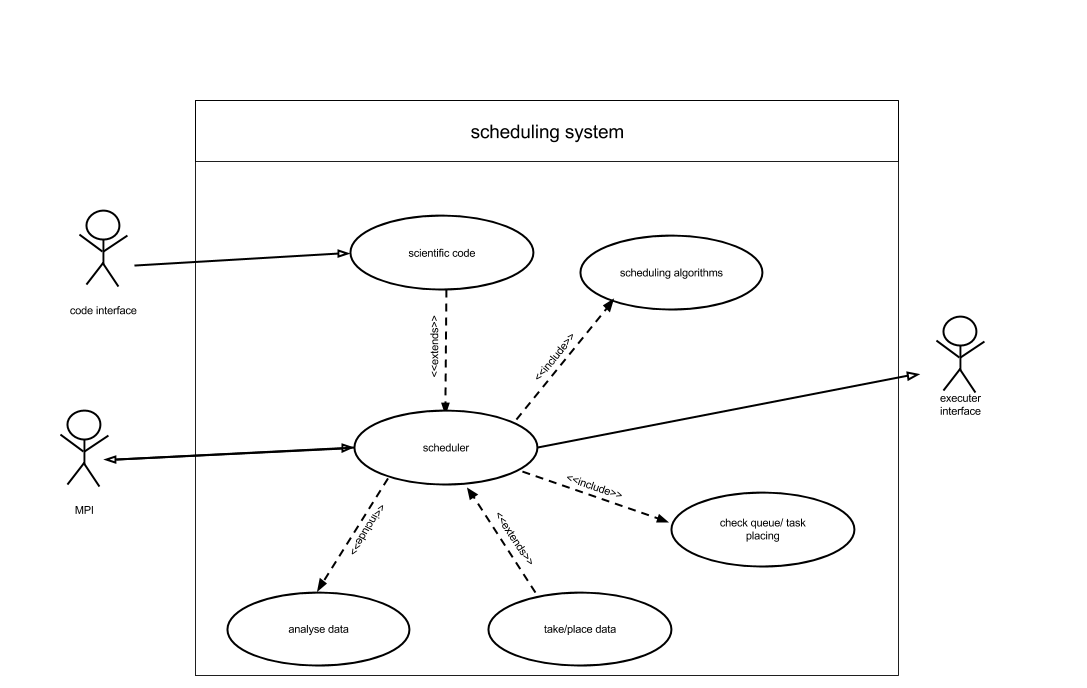
\includegraphics[width=1.5\textwidth,scale=0.75,trim=7cm 0 -7cm 0]{images/usecasediagram.png}
		\caption{Activity diagram}
	\end{figure}

\title{Task Stealing (Nice to have)}

\begin{enumerate}[1. ]


\item Brief Description
\newline
This use case describes the way a task stealing algorithm works inside a dynamic scheduler in order to reduce the amount of process migration between processors.

\item Actors
\newline
No actors. 


\item Preconditions
\begin{enumerate}
\item The scheduler has been initialized and it has already created a MPI memory window for RMA (Remote Memory Access).
\item Information about initial tasks has been collected from code preprocessing, received tasks from which have been placed to the queue.
\end{enumerate}

\item Basic Flow of Event
\newline
The use case begins when the scheduler checks if there are tasks in its own queue.If there is a task in the queue, it will be executed. After the task has been executed, all collected results will get placed in the database in an organized manner.
If there isn't any task in the queue, the task stealing process will be initiated. First of all, the scheduler will cycle through all running processes in other processors and try to steal an idle task from them. In order to check the other processes' queue for an idle task, the scheduler tries to block the RMA window for offsets and statuses, after which it checks whether there are any idle tasks. If the queue is empty or if the RMA window is currently blocked, the scheduler repeats the same procedure for remaining processors. If after checking all processes, no idle task was found, the scheduler changes its own state to idle. If this idle state doesn't change for a specific amount of cycles, which means that no tasks were stolen in this period, the scheduler finally checks to make sure that no process is currently running in any processor and if that's the case, it finishes its own routine. 


\item Post-conditions
\begin{enumerate}
\item The scheduler frees the allocated MPI memory window for RMA.
\item The scheduler executes the finishing post processing routine, where it collects information from the whole process (e.g. global total run time).
\end{enumerate}

\item Special requirements

\begin{enumerate}
\item The scheduler should have access to the executer interface.
\item The scheduler should be accessible through an interface, in order to receive new tasks from the code interface.
\end{enumerate}

\end{enumerate}

\subsection{Object model}
\title{Basic module diagram}
\newline
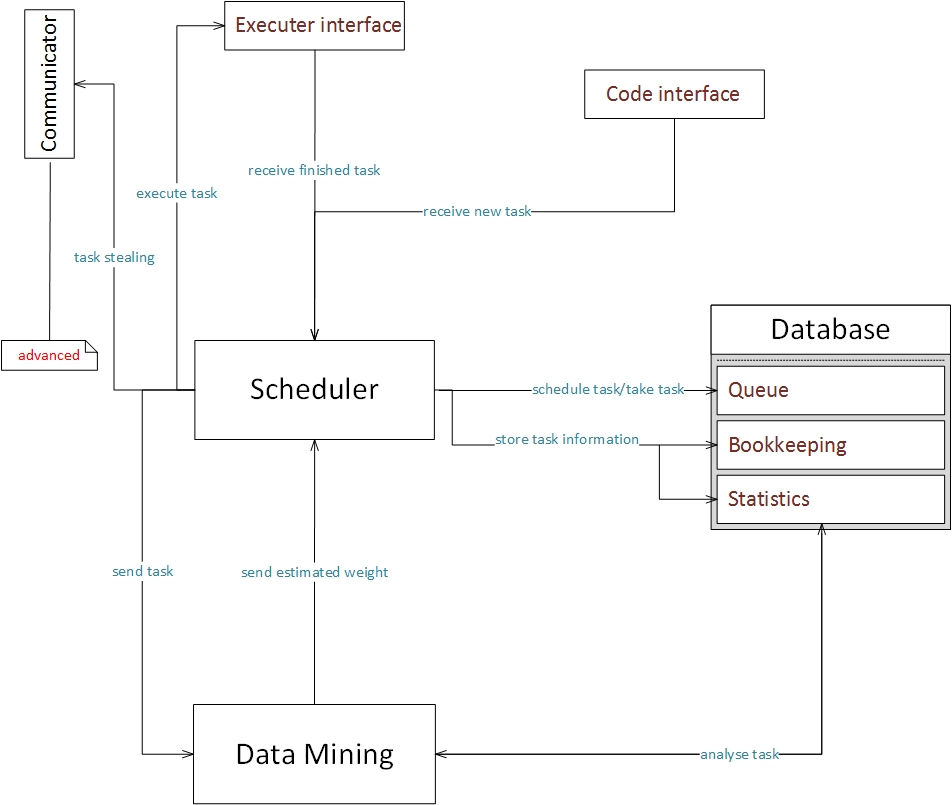
\includegraphics[width=15cm]{images/modules.jpg}
\newpage
\subsection{Dynamic models}

\begin{itemize}
\item Sequence diagram \newline
	\begin{figure}
	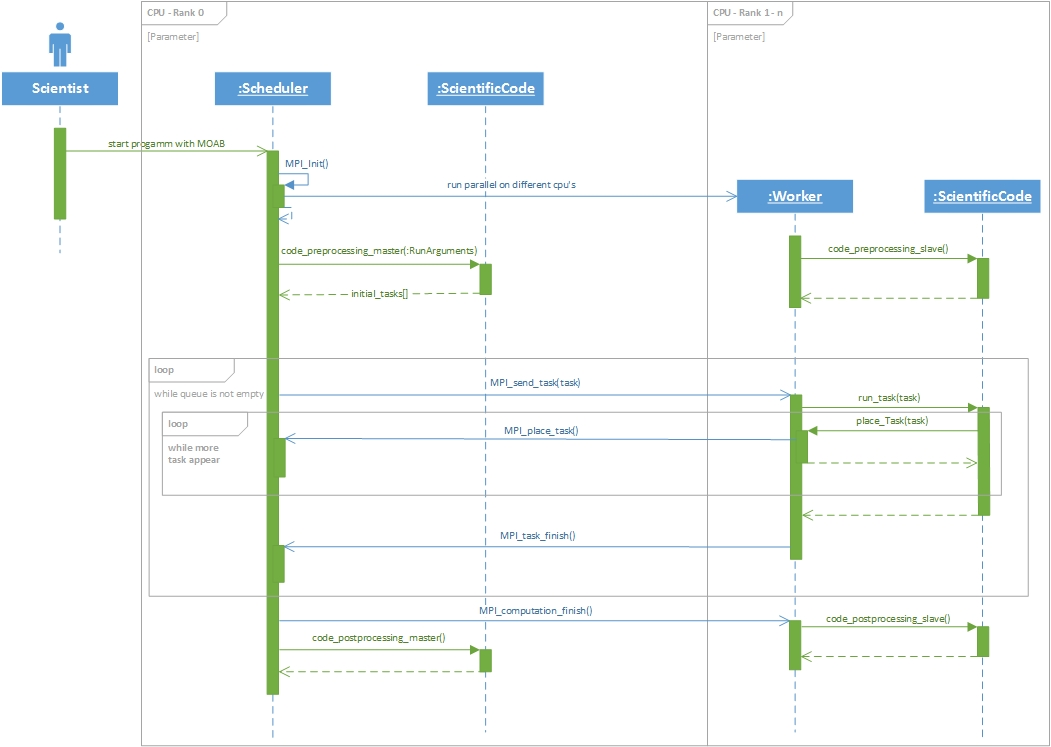
\includegraphics[width=15cm]{images/Master-slave.jpg}
	\caption{Master-slave diagram} 
	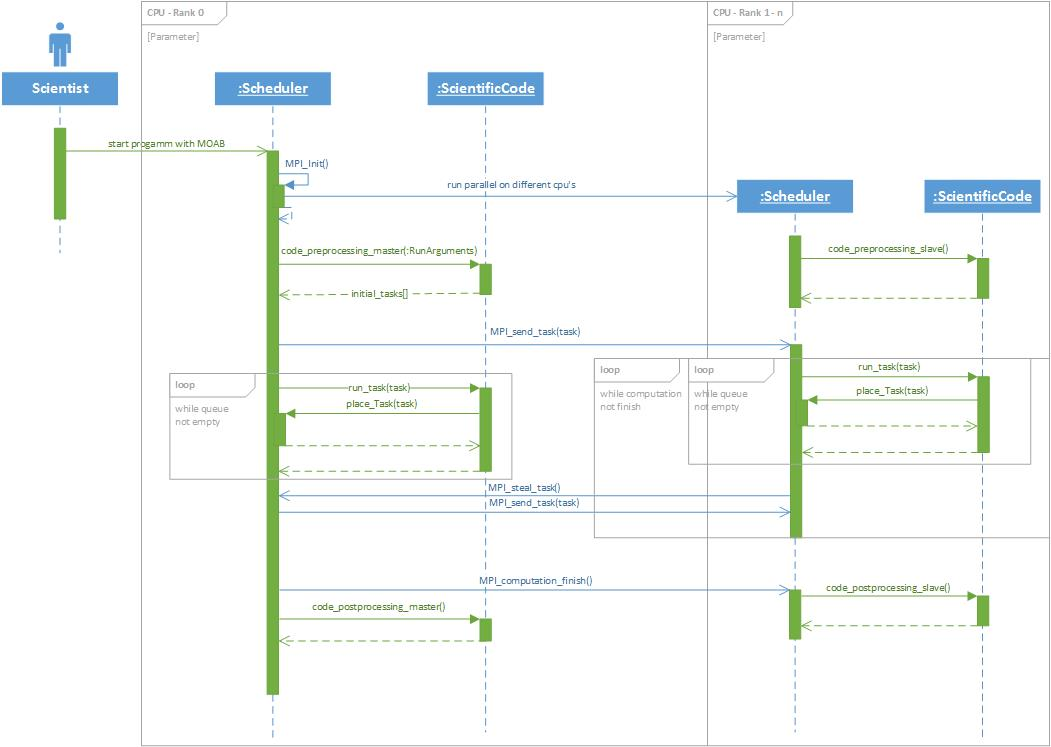
\includegraphics[width=15cm]{images/Task-stealing.jpg}
	\caption{Task-stealing algorithm}
	\end{figure}
\end{itemize}
\subsection{Graphical user interface}
			maybe
	\section{Glossary}
\begin{description}
	\item[CLI] Commandline interface
	
	\item[Master-Worker] There is one Master scheduler which schedules the tasks. The other instances are the workers. Its the opposite of Mutiple-queue.

	\item[Nodes] The bwUniCluster is devided into 522 nodes which have 16 to 32 cores with 64 to 1 TB main memory and 332,8 to 614,4 GFLOPS for more information please visit \href{https://www.scc.kit.edu/dienste/bwUniCluster.php}{https://www.scc.kit.edu/dienste/bwUniCluster.php}

	\item[Multiple-queue]Each scheduler has its own queue. All schedulers are equal and use task-stealing to avoid idle. Its the opposite of Master-Worker.

	\item[GFLOPS] 1 GFLOPS means $10^9$ flotingpoint operations per second

	\item[Moab workload Manager] Moab provides numerous interfaces allowing it to monitor and manage most services and resources. It also possesses flexible interfaces to allow it to interact with peer services and applications as both a broker and an information service. This appendix is designed to provide a general overview and links to more detailed interface documentation

	\item [SimLap for Elemantary- and Astro-    Particle Physics (SCC)] Support scientific groups with concept „S.P.O.R.A.D.I.C. services for simulations“ (Standardisation, Parallelising, Optimization, Release, Adaptation, Data Intensive Computing) \href {https://www.scc.kit.edu/en/research/7047.php}{https://www.scc.kit.edu/en/research/7047.php}

	\item[MPI-world] The comunication enviroment which is used by the scheduler to comunicate with each other 

	\item[Data mining] The process to extract useful information from a big amount of data

	\item[Scheduling strategies] The programm provides multible strategies to schedul the tasks

	\item[Scientific code] The code the user wants to execute
	
	\item[HBC] Shortcut for high-performance computer(supercomuter)
\end{description}
	
	
\end{document}
